\documentclass[a4paper]{article}
\usepackage{amsmath}
\usepackage{amssymb}
\usepackage{geometry}
\usepackage{enumerate}
\usepackage{float}%稳定图片位置
\usepackage{graphicx}%画图
\usepackage{wrapfig}
\usepackage{indentfirst}%缩进
\usepackage{enumerate}%加序号
\usepackage{multirow}%合并行
\usepackage{subfigure}
\usepackage{graphicx}
\usepackage{hyperref}
\usepackage[bottom]{footmisc}
\usepackage{listings}
\usepackage{xcolor}
\title{\Large \textbf{Robot for the Combat Against Covid-19: A Systematic Survey}\\
\author{\textbf{}\\
\emph{University of Michigan Joint Institute, Shanghai Jiao Tong University, China}\\
\date{}
}
}
\begin{document}
\maketitle
\section*{\centering Abstract}
    This systematic review aims at providing valuable information and conclusion about robot's application in fighting Covid-19. The review searched nine databases for relevant studies with specific keywords, and then extract and analyze data from selected articles. The main content covered by these articles is about robot application under pandemic as well as feedbacks from former experiments. The review provides a comprehensive summarize on these documents by highlighting robots' features as well as pointing out their drawbacks. It is found that telepresence robot is a rapidly growing field, and it has been put into use in many scenarios during quarantine.
\emph{Keywords:
Telepresence robot, healthcare robot, Education robot, Industrial robot
Robots for Corona Virus management}
\section{Introduction}
    The world are facing one of the most serious pandemic in the last 100 years. Until June.2nd, 2020, Covid-19 virus has infected more than 6 million people and killed nearly 400 thousand patients all over the world. There are 216 countries, areas or territories with cases and fighting against it\cite{1}.
\begin{figure}[H]
    \centering
    \includegraphics[scale=0.15]{map.png}
    \caption{WHO Covid-19 Dashboard}
    \label{Map}
\end{figure}
    It is predicted that the number will keep increasing and we have to fight against the virus for a long time. What's worse, the pandemic also have hurt the global economy badly. According to International Monetary Fund's prediction, the global economy will shrink by 3\% in 2020\cite{2}. The economic stress may badly affected the production of medical resources including protection suits, masks, and goggles. Lack of medical resources is a key factor for the large number of infected medical professionals. According to statistics, more than 2\% of the patients are nurses or doctors. Most of them were infected when treating other patients.
\par 
    Therefore, we need to take measures to reduce the number of infected people as much as possible as well as protect those who haven't been infected. The key step to stop the virus from infecting people is to reduce people's close contact. Letting robots do human's job can be an effective solution since they won't get infected during work. With development of robotic technology and artificial intelligence, people have already designed and produced several kinds of robots. Many of them are already being put into use and doing specific jobs for human now. In hospitals, ICU robots and nursing robots are helping provide remote treatment for patients. Some general robots including service robots, teleconference robots, and telepresence robots can also play an effective role under current situation. With help from robot, face to face meeting can be held online, and medical professionals won't be at risk of being infected when treating patients. Robots can greatly save our manpower and materials resources as well as lower medical professionals'.
\par 
    This research will perform a review by analyzing robot's usage and features for fighting against Covid-19 virus. Afterwards, the review will classify these robots, point out their drawbacks, and propose suggestions for further improvements. The systematic review will mainly focus on a robot's: 
\begin{enumerate}
    \item Function.
    \item Scenario for application.
    \item Drawback.
    \item Further improvement.
\end{enumerate}
\section{Methodology}
    This systematic review is based on the method called Preferred Reporting Items for Systematic Reviews and Meta-Analyses (PRISMA)\cite{99}.
Figure.\ref{PRISMA} shows the four phases of PRISMA, including identification, screening, eligibility, and included. 
\begin{figure}[H]
    \centering
    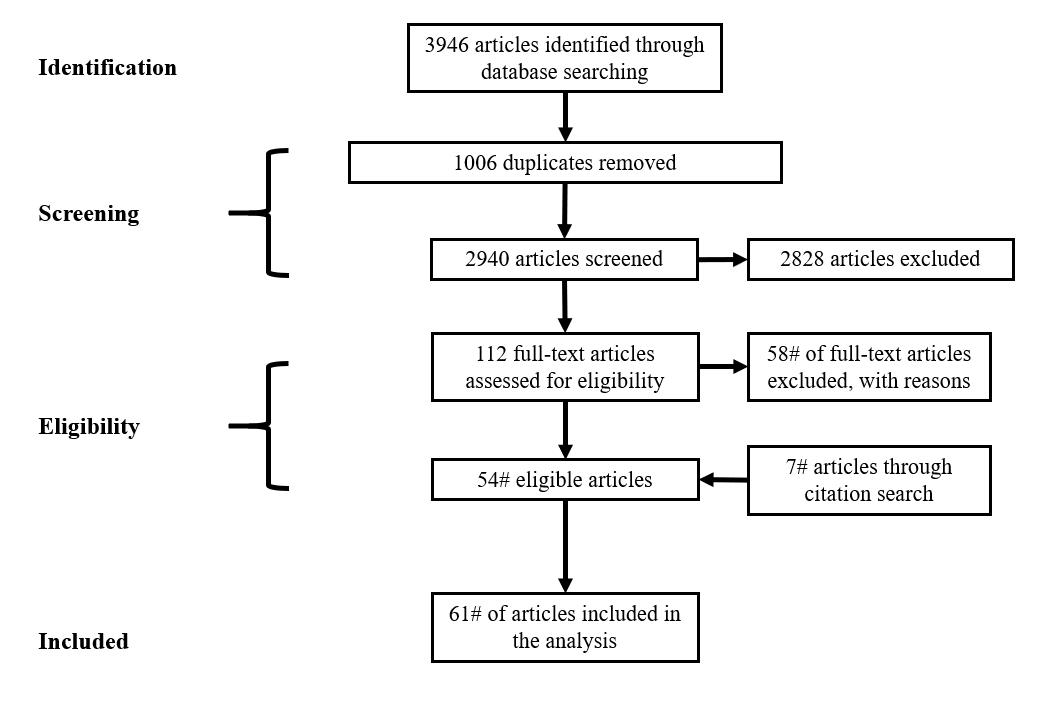
\includegraphics[scale=0.2]{PRISMA.png}
    \caption{PRISMA Process}
    \label{PRISMA}
\end{figure}
\subsection{Identification of Resources and Search Terms}
    This review selects scientific articles from electronic databases and citation researches of selected articles. 
Nine electronic databases including (CINAHL, ERIC, EMBASE, IEEE Xplorer, MEDLINE, Proquest Central, PubMed, PsycINFO, and Web of Science) are accessed. They are most frequently used by scientific researchers and provide a large number of deep scientific research articles. To make this review as comprehensive and relevant to this review's objection as possible, keywords are split and connected through boolean connectors \textbf{AND, OR}.
\par 
    The search term is \textbf{robot AND (Covid OR pandemic OR quarantine OR teleconference OR epidemic OR telemedicine OR telepresence)} and the search field mainly includes title, abstract, keywords, and subject. This review only covers articles published from 2010 to 2020 in English because robotic technology was not mature enough before 2010. 
\subsection{Search Result}
    In total, 3946 articles were retrieved, and they're all stored in EndNote (A commonly used bibliography reference manager). Figure.\ref{Database1} shows their distribution among different databases. 2940 articles remained after 1006 duplicates with the same title were removed.
\begin{figure}[H]
    \centering
    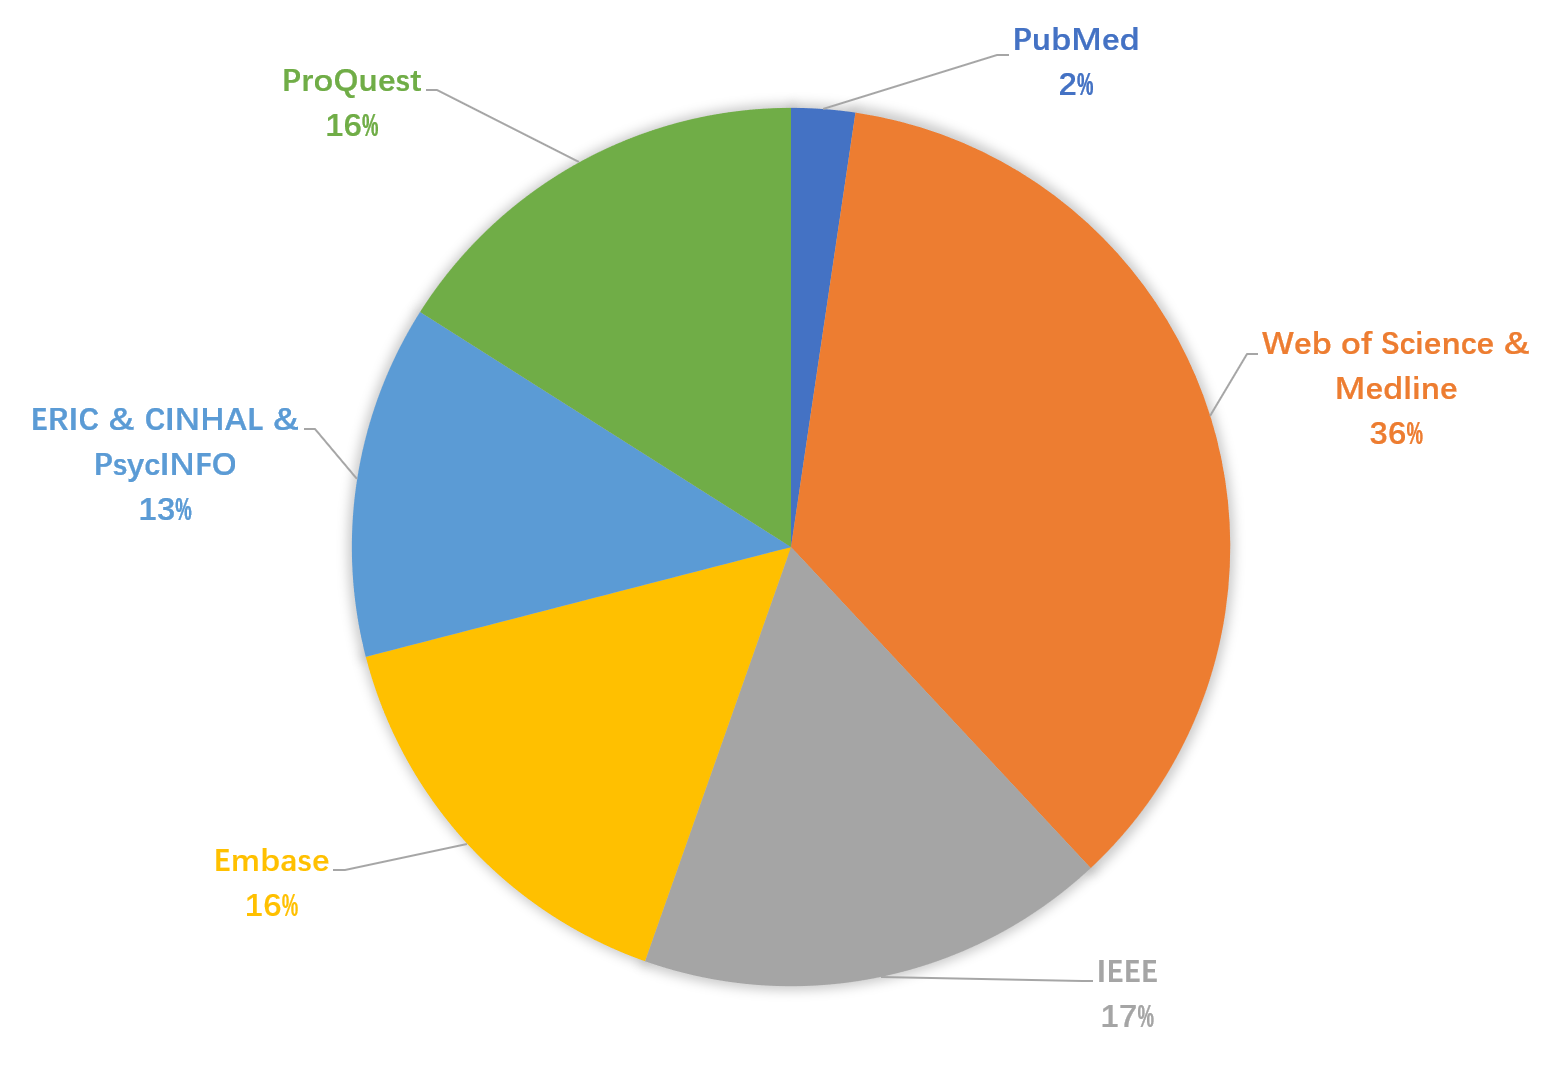
\includegraphics[scale=0.15]{Database.png}
    \caption{Database distribution}
    \label{Database1}
\end{figure}
\subsection{Selection of Relevant Articles}
    To narrow down the search results and select articles relevant to pandemic management, we assess eligibility of articles by scanning the title, abstract, and keywords. 2828 articles are removed because one of following reasons:
\begin{enumerate}
    \item Focus on theory or algorithm rather than functions or applications of some robot.
    \item Clearly can't offer specific help during the pandemic.
    \item Lack essential publication information  . 
\end{enumerate}
    In next stage, the investigator reviewed the remaining 112 full-text published articles for their relevance to the objective of this systematic review. 54 articles were included since they provide enough information about robots which have potential to be used for Covid-19 management. Subsequently, 7 articles from the bibliographies of selected articles were included. Totally, there are 61 articles selected for the systematic review. 
\subsection{Data Extraction and Analysis}
The investigator extracted the following information from 61 articles included in the systematic review:
\begin{itemize}
    \item Aims and objectives
    \item Type of documentation and its Methodology
    \item The robot's application scenario during pandemic.
    \item The challenge, drawback and improvement orientation of the robot. 
\end{itemize}
\section{Results}
\subsection{Type of documentation}
    According to objectives and methodology, each article is classified into four types of documentations:
\begin{itemize}
    \item Quantitive and qualitive studies.
    \\Almost all studies use mix-methods in their experiments. In this review, we classify studies which use a large scale of quantitive analysis as quantitive studies. They mainly use data analysis to get a persuasive conclusion. On the contrary, qualitive studies focus on interview with users and their feedback. Both kinds of studies are about robot performance during experiment or application. They can provide concrete and summative conclusion based on experiments or interviews, which expose the robot's drawbacks and problem.   
    \item Technical reports.
    \\The technical reports gives a comprehensive introduction about how a robot was designed and manufactured by describing the design and concrete usage of each function. Case studies with mix methods are also included to test the robot. Even though robots in these reports are usually not mature enough for application, they have a higher potential and more room for further improvement.
    \item News reports  
    \\News reports mainly discuss robots' specific usage under current pandemic. By showing the practical applications in different scenarios, the reports can bring more ideas to determine a robot's orientation for future development or improvement. In addition, these studies also show the social acceptance and attitudes for robots. 
\end{itemize}
    Figure.\ref{Documentation type} shows the distribution of articles in each category. Quantitive and qualitive studies are the majority of these articles. Close number of each kind of studies are included, meaning that interview and data are both effective feedbacks for experiments. Technical reports are published in different years, showing that even a robot developed a long time ago can currently help people release pressure from the virus. In contrast, the news reports mainly focus on the present, about how robots are being applied in fighting against Covid-19. 
\begin{figure}[H]
    \centering
    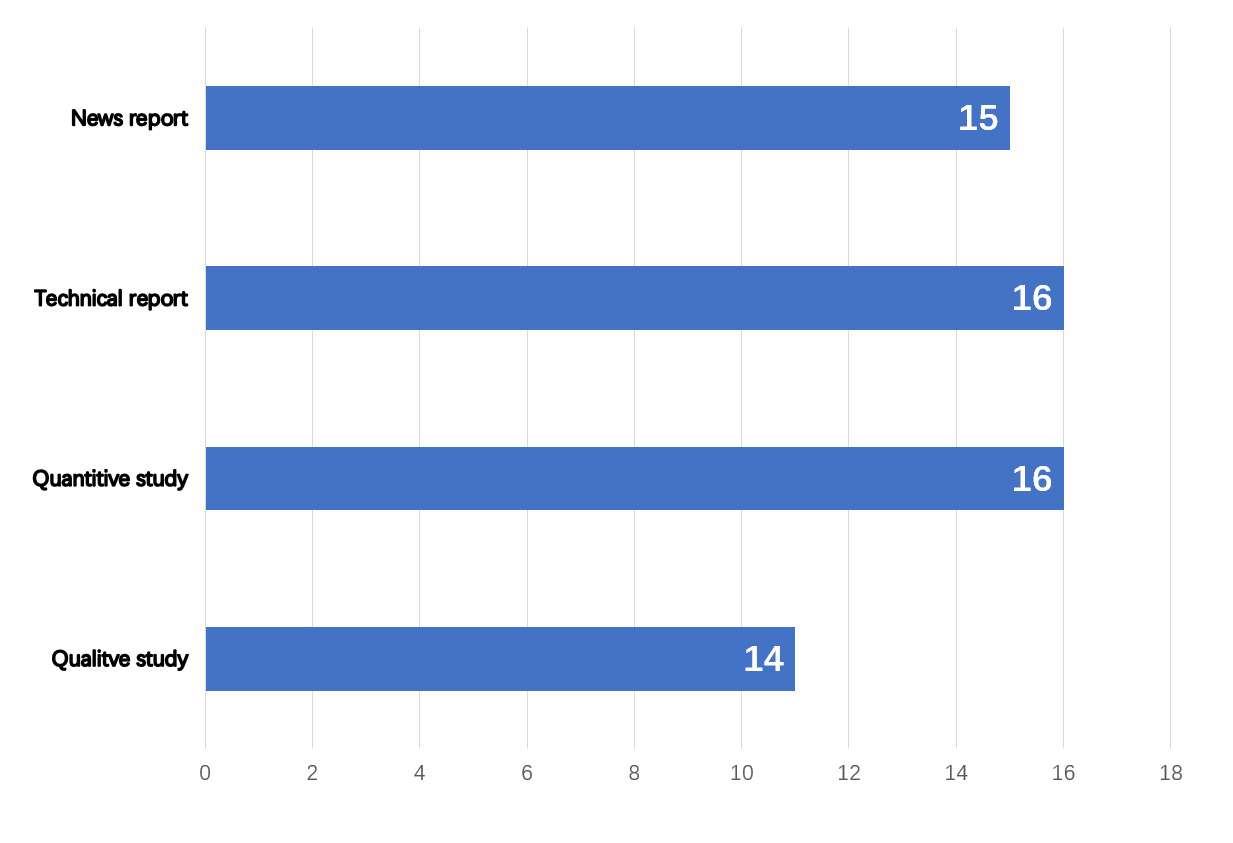
\includegraphics[scale=0.25]{Type.png}
    \caption{Documentation type}
    \label{Documentation type}
\end{figure}
\subsection{Demographic}
\begin{figure}[H]
    \centering
    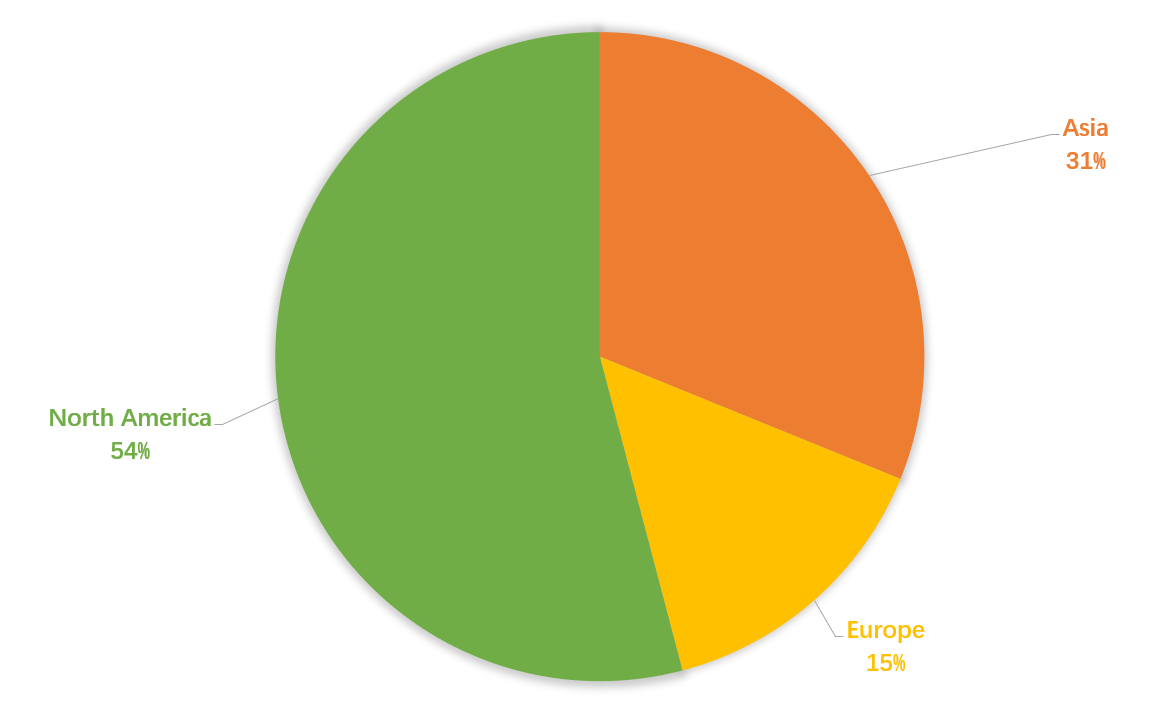
\includegraphics[scale=0.2]{Demographic.png}
    \caption{Documentation type}
    \label{Demographic}
\end{figure}
    There are 54\%(33/61) articles from North America, 31\%(19/61) articles from Asia, and 15\%(9/61) articles from Europe. The continents have a close number of case studies.  Asia has most technical reports. It's probably because there is a large market for robots at Asia. North America has the most news report because the pandemic situation is worst there now. 
\subsection{Analysis Based on Applications }
The selected articles are classified into four categories based on the application scenarios for the robots discussed.
\begin{figure}[H]
    \centering
    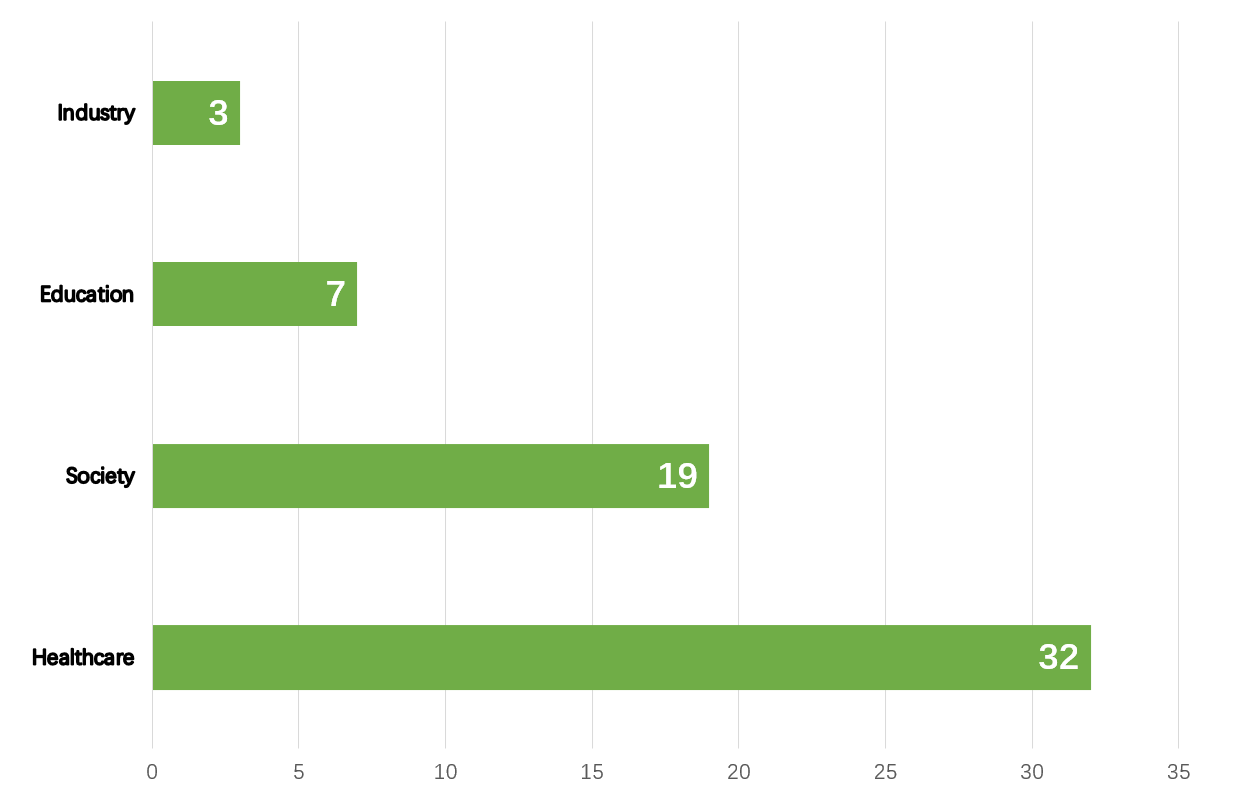
\includegraphics[scale=0.2]{Application.png}
    \caption{Application}
    \label{Application}
\end{figure}
Figure.\ref{Application} shows the articles' distribution according to their robot's applications.
\subsubsection{Healthcare Applications} 
    Nearly half of the articles' focus on the healthcare application of robots, which can play an important role in medical treatment. Actually, robots have been utilizing in the medicinal business from the past over two decades\cite{3}. They may have different backgrounds and own features, including performing medical procedures, dealing with the patients, drug store, nano robots, small scale robots, clairvoyance, restoration and other work zones. Among these robots, hospital and ICU robots, medical consultation robot, pandemic management robots, and care robots are the main force to help human fight against Covid-19.
\paragraph{Telepresence Robots}
    Telepresence robot is a new area which have developed rapidly in the last decades. They're generally 1-1.6m high, equipped with a remote control system, a camera, a tablet, and a mobile system. The users of telepresence robot are controllers and occupants. The controllers can be doctors, caregivers or anyone who control the robots, while the occupants include patients or the elderly, who are the service object of the robot. The remote control system enables the controller to operate the robot from a distance. The camera and tablet provide visual and audio channel for the controller to supervise the environment and communicate with occupants. With the mobile system, the telepresence robot can work as a substitute of the controller to perform an action or move to somewhere. 
\par 
    Generally, the robot and the controller are connected to each other through Internet. The controller can use computer or cell phone to give instructions to the robot as well as see the video recorded by the robot's camera. For an advanced control system, even an inexperienced controller just needs to take a while to learn how to control the robot smoothly\cite{4}. On the other side, the controller's image will also be shown on the tablet installed on the robot, which will be seen by the occupant. It is worth mentioning that the robot can be fully controlled by the remote controller, including initialization. As a result, the occupant, even a totally ill abed patient, can communicate with the controller through the robot without doing anything.  
\par 
    As early as 12 years ago, telepresence robot has already been on trial during the Great California Shakeout, a drill with involved multiple agencies. The telepresence were responsible for providing remote triage and treatment consults of victims. During the drill, the robot was proved to be a useful means to extend resources and provide expert consult if specialists were unable to physically be at the site\cite{5}. At present, telepresence robot can provide more diversified services, including telecheckups, telemonitoring by recording physiological data, teleconsultation, and teletreatment and etc\cite{6}. Therefore, it has a high potential to be popularized in healthcare and other field.
\paragraph{Hospital and ICU robots}
    In hospital, a lot of medical professionals are infected due to close contact with patients and lack of masks or protection suits.  On the other hand, healthcare workers in quarantine wards in hospitals may feel fatigue to perform periodic routine checks specially to take adequate measures like disinfecting the area, putting mask etc. every time they enter the ward. Telepresence robot can overcome the unavailability of eminent medical personnel as well as relieve their fatigue during threatening emergencies\cite{7}. One robot can make the rounds of the wards and doesn't need a mask or protection suit. For nursers and doctors, they can sit before the remote control station and monitor the process by just viewing the screen and click the mouse.
\par 
    A robot called A-8mo has already been touring the rooms at the Hospital San José and giving telepresence consultations to patients confirmed with Covid-19 virus. This form avoids the risk of contagion and saves protection supplies\cite{8}. A-8MO allows the doctor to make a virtual consultation in real time, facilitating interaction without unnecessarily exposing the health professional. The robot also has two cameras and six microphones to make sure the communication between patients and doctors is smoothly enough. By expanding robots like A-8MO to other hospitals, front-line nurses can work more like a system administrator\cite{9}.
\par 
    In areas where the pandemic is very serious, there are a lot of critical patients, who can only receive treatment in the ICU. These patients will occupy a huge amount of medical resources, including 24-7 care, a breathing machine, and a whole team composed of experts in different medical fields. Given the acknowledged shortage of intensive care specialists and their critical condition, it requires the bedside nurse to have real-time access to senior level intensive care physicians, and conversely it requires the physicians to have access to the intensive care unit\cite{10}. ICU robot is a kind of telepresence robot specially designed to handle this situation. 
\par 
    For care providers, ICU robots enables fast face-to-face communication between them when they are not present in the ICU. Unlike old-fashioned telephonic communication, care providers located remotely can also observe patients' vital signs, examine medical charts\cite{11}. For senior physicians, ICU robots free them from being busy coming back and forth between wards and improve their work efficiency. For Covid-19 patients, CT image is the most direct basis to analyze their condition. Bedside nurses can transmit the CT image to senior physicians through ICU robots so that they can acquire detailed and full understanding of a specific patients' condition remotely. 
\begin{figure}[H]
    \centering
    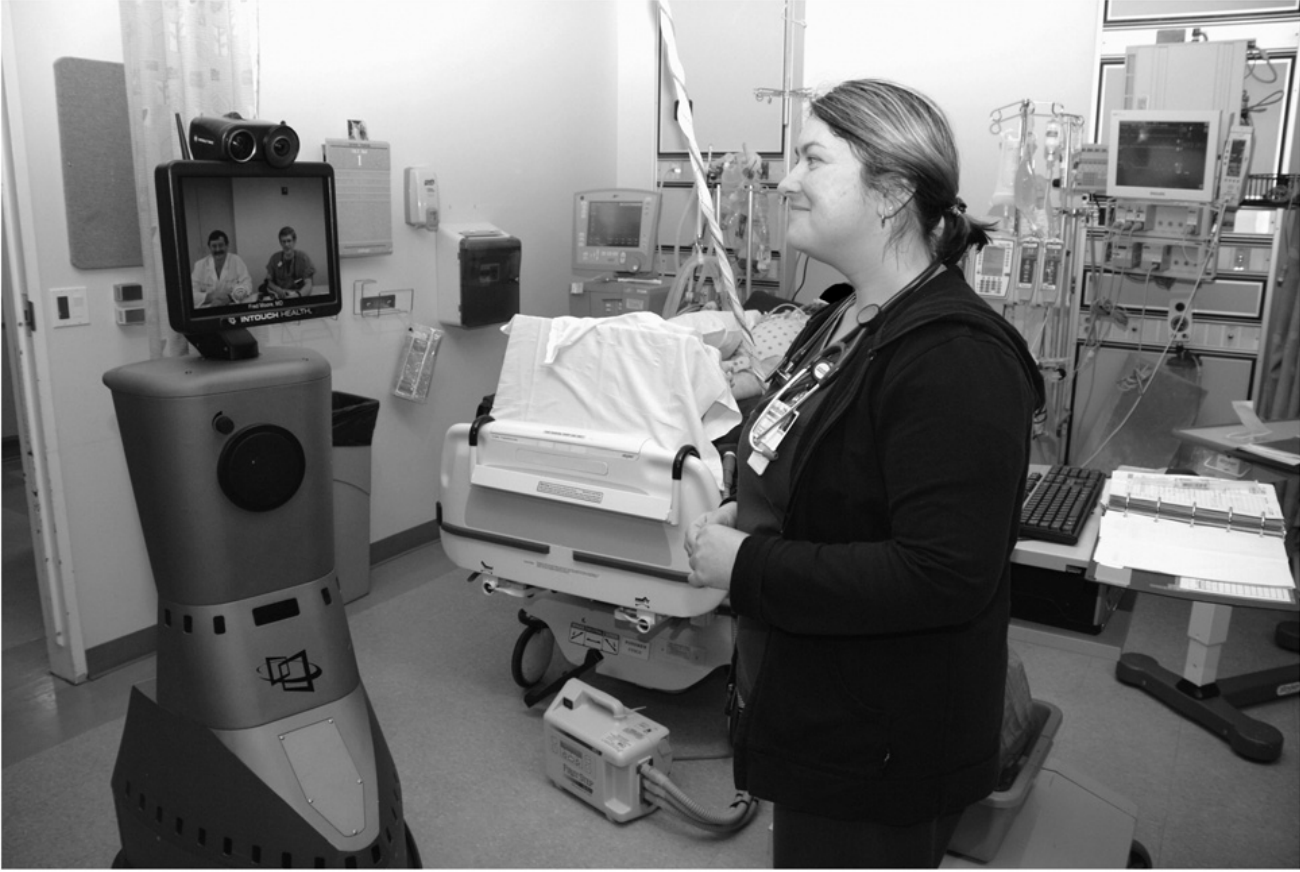
\includegraphics[scale=0.2]{ICU.png}
    \caption{A group of medical experts are using an ICU robot to make remote diagnosis}
    \label{ICU}
\end{figure}
\par 
    A conceptual framework proposes to use the robot as a surrogate on the unit to replace having the entire multidisciplinary team standing at each patient's bedside\cite{12}. The team members take turns to control the ICU robots to make a very detailed diagnosis from different aspects. The robots enable them to view others diagnosis and share their results. Afterwards, the team members can collaboratively make a decision on future treatment through video meeting. This framework can facilitate the collaboration between medical experts from different fields as well as improve their efficiency. Hospital can set multiple stations at in many places, including the ICU, emergency Department, and postanesthesia care unit or on the general medical or surgical wards\cite{13}. When there is a emergency, even though the medical professionals are scattered all over the hospitals, they can quickly go to their nearest control station respectively and start the remote diagnosis. 
\par 
    According to feedback from clinic test, more than 75\% patients and medical professionals agree that ICU robots can provide satisfying medical service. We have full confidence that ICU robots can greatly ease the burden at places seriously hit by the pandemic.
\paragraph{Care Robot with IoT}
    The pandemic also has caused much inconvenience for normal people, especially for the elderly and disabled. They can't receive regular medical treatment and care because hospital is the hospital is the most dangerous and busy place. Because of quarantine, it's also difficult for their family or private doctor to visit them. Care robots can help them through the difficulties. Compared to medical robots in hospital, these robots support multiple language and can be used at home. The main occupants of care robot are those who are isolated at home. Care robot is equipped with a clear camera and advanced tablet to focus on providing spiritual and physical care service rather than doing nurses' job at hospital. In addition, care robots can work with some sophisticated devices for telediagnosis. A remote auscultation robot enables the doctor to listen to the noise from the stethoscope thanks to a diaphragm and a headset where the audio stream from the patient site is played\cite{14}. The robot can transmit the noise at a very high resolution so that the doctor can examine the circulatory and respiratory systems namely heart and breath sounds as well as the gastrointestinal system namely bowel sounds. Some care robots can be connected to the Internet of Things as an intermediate station to work together with sensors, cell phone, TV, etc\cite{15}. When the occupants require telemedicine service, the doctor can use the robot to set up connection with other medical equipments in patients' home for a detailed diagnosis. For example, the doctor can use the robot to connect an electronic thermometer in the patient's home and check his temperature. 
\par 
    Care robot also performs well in providing interpersonal communication for people in isolated environment\cite{16}. In addition to making a video call, the advanced tablet enables users to run some interactive applications, which can greatly relieve occupant's loneliness during quarantine, especially for the elderly or disabled. Through IoT, care robot can also be connected to a smart TV or teapot so that the controller can play a program on TV or make tea for the isolated occupant.
\par 
    Even when there is no controller, care robot can offer much help by itself. Some robots can monitor the heart rate and body posture of people. When there is an accident like the elderly tumbles, the robot recognizes the danger and alarms their families or doctors\cite{17}. Others can determine what skin disease the patient has just by scanning the photos\cite{18}. Various kinds of care robots have already been put into use in many countries and it is a good way to give consolation to people isolated at home.
\paragraph{Public Use}
    In public area, robots are doing everything from bathing surfaces with radiation, sanitizing floors, scanning for fevers, spewing anti-microbial gas and enforcing mask wearing \cite{19}. For outdoors disinfection, robots are attached a disinfectant sprayer so that it can spray in public places. They can also dispense germ-killing fluid from its tanks. Since the outbreak of the Covid-19, the demand for UV light disinfecting robot has increased rapidly, thanks to its high efficiency in indoors disinfection. Xenex Disinfection Services LLC has developed broad spectrum, high-intensity ultraviolet light technology which enables one robot to disinfect a room in two minutes\cite{20}. The robot can clean dozens of rooms a day, catching microscopic bacteria and viruses often missed by a manual cleaning process. 
\par 
    Besides disinfection, robots are being used to remotely detect suspected Covid-19 patients. They can work round-the-clock in all airports, outlets, shopping centers, hospitals, clinics, universities, schools, metro stations, and crowded places\cite{21}. The robots operate as a sanitary filter in buildings and other facilities that have put security guards to take the temperature before allowing entry. An advanced humanoid robot called Roomiebot has been implemented in Mexico, seeking to reduce the first contact between potential Covid-19 patients and healthy people. It can move automatically and use an oximeter to identifies whether the person has shortness of breath\cite{22}. In addition, it can interact with people to request people to perform a questionnaire about the symptoms of the disease and measure the temperature\cite{23}. With sophisticated camera and contactless temperature sensors, the robot can detect body temperature from a distance or precisely detect Covid-19 symptoms, including fever, cough, heart rate, temperature, and humidity. Compared to human detector, a robot can use its camera to detected multiple people's temperature at the same time and upload the image and results to the control center, which is more efficient. There is no doubt that these robots can greatly save human resources in public areas.

\paragraph{Inefficient Power System}
    Since a robot have various functions, it also need a strong power system. However, battery life is a common issue for all mobile devices. Giraffe is an advanced robot that have already been tested in the elderly people home. However, many primary users have concerns on Giraffe's electrical consumption\cite{24}. An experiment shows that Giraffe can only work for two hours and it needs another two hours to be fully charged\cite{25}. On the other hand, the power system may overheat after functioning for a long time continuously, and hence it needs a powerful fan for heat dissipation. However, the fan usually has a loud noise, which ruins the user's experience. In the future, the developers need to increase the power efficiency of the robot so that the robot can function at a quieter status for a longer time. Adding a back up battery on the robot may be one method to extending the battery life\cite{26}. 

\par 
    Many developers have already generated and applied the idea of automatic charging. Experiments and feedback from users also prove the significancy of this function\cite{33}. Old users are likely to forget to charge the robot or feel difficult to handle the manual charging system, while medicine professionals are usually too busy to pay attention to the battery status. A automatic charging function can improve the continuity as well as the usability of the robot.

\paragraph{Large Size}
    For telepresence robot, to make sure the users can see the tablet clearly, it's just a bit lower than a normal person. As a result, a big chassis is necessary to prevent the robot from falling down during work. However, the big body also adds inconvenience and safety concerns\cite{27}. It can increase the possibility for the robot to hit a obstacle or cause an accident. In places like wards or a  small room, the robot may also have space conflict with other medical devices and healthcare providers.
For disinfecting robot, it is possible that the idea of autonomous robots that clean may lose some of its glimmer after the Covid-19 fades. The robot may turn out to not be cost effective, compared to traditional manual labor. Not to mention it's much tougher for robot to reach some surfaces like door handles than human. As a result, there are expectations that disinfecting robot in the future will have a smaller form to lower the cost and improve its flexibility.

\paragraph{Unsatisifying Performance at Night}
    A study has shown that the physician may favor robot over the normal telephone during nighttime rounding because of the possibility for face-to-face communication with both residents and nurses\cite{28}. However, when  night emergency happens in the hospital, the robot can't achieve the same performance as in daytime. The main reason is the lack of light, which makes it inconvenient for the medical professionals to view the surrounding from the robot's camera. The solution can be adding a flash light or night vision model to the robot, but the light may disturb others and the night vision model puts forward higher requirements for nurses' driving skills.

\paragraph{Unstable Signal Transmission}
    On the other hand, the stability and efficiency of network signal transmission is extremely important because there is a long distance between the controller and the telepresence robot. The instability may cause delay or unavailability in remote control and video call, which may lead to more serious accident. For example, a robot may keep rushing forward and hit someone because it doesn't get an instruction to stop. Therefore, developers must make the control system as stable as possible and provide emergency control function. Some studies have proposed different architectures for stable signal communication, but they still need time to prove its practicability in long range control.

\paragraph{Integration of the Computing Power}
    Up to now, healthcare robot's applications are still very limited, and it still has many functions remain to be developed. For example, the mobility of the robot is only limited in space, but it can be broadened by artificial intelligence, machine learning or Internet. The tablet equipped on the robot has a strong computing power, but they're rarely used to collect, record, and analyze the patients or disease's data. A smart diagnosis architecture with four stages is proposed to integrate the the computing power together with remote control\cite{31}:
\begin{enumerate}
    \item The robot first comes to the patient and takes measurements through the comprehensive medical sensors consist of physiological, pathological and in-body imaging.
    \item All these measurements are fed to the anomaly detection module that derives critical information mostly related to abnormalities of the measurements. 
    \item The job of this cognitive engine is to relate this set of anomalies to possible disease and send the report to doctors/hospitals for their use.
    \item The robot can automatically search the Internet for related information for future treatment.
\end{enumerate}
    This architecture has already been tested in an experiment, and it shows it can work effectively.
\paragraph{Development in Transportation Function}
    The high mobility of the robot have not been fully applied as well. The powerful chassis of the robot can help transport a patient or people with disabilities\cite{32}. Figure.\ref{Transportation Robot} shows a prototype of one stretcher robot. The robot can send patients to the ward without man's help.
\begin{figure}[H]
    \centering
    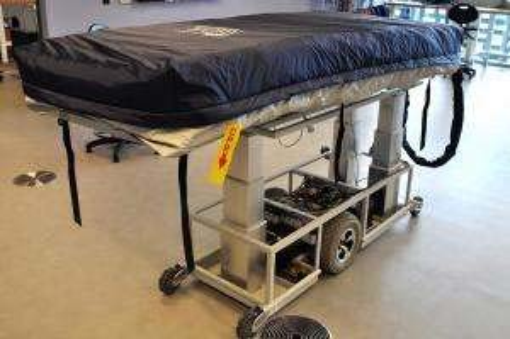
\includegraphics[scale=0.25]{Transportation.png}
    \caption{Transportation Robot}
    \label{Transportation Robot}
\end{figure}
    New version of medical transportation are under development. The robot is expected to be able to monitor the patient's vital signal and provide essential life support during transportation. When it comes to biped robot, it can transport patients very quickly when there is a stair. Medical transportation robot is more like traditional industrial robot, but it can an important member of the medical team and save many lives.

\paragraph{Requirement for Voice Control} 
    According to feedback from an experiment about telepresence robot, controllers believe that an improved control interface can make their experience better, especially for care robots. In addition, many users hope that the robot can support voice control in the future. The primarily occupants of remote care robots are usually in bed or not very familiar with how to use an electronic devices. The voice control enables them to enjoy the robot's service without making physical contact or dealing with the dazzling user interface. For busy medical professionals, the function allows them to give instruction to the robot and do their work simultaneously. Voice control has been proved useful in mobile phones, it can also make the robots more user-friendly.
\paragraph{Harmelss Disinfection} 
    When it comes to disinfecting robot, if the UV light won't do any harm to human, then the disinfection will be more popular and convenient because it won't interrupt people's work any more. On the other hand, people hope the new generations of large, small, micro-, and swarm robots that are able to continuously remove dust and truly sanitize all surfaces could be developed\cite{34}.

\paragraph{Lack of Trust}
    There are significant differences between users and nonusers in their attitudes to ICU robots. Almost all medical professionals have used ICU robots felt more confident caring for the patient with the supervising physician observing the visit via the ICU robot, compared to only 10 percent of the nonusers. The difference reflects that medical professionals' first impression for robots is distrustful, and they won't change their attitudes until they have a actual trial on it. 
\par 
    It's worth to mention that the distrust is bilateral, the patients also have an initial prejudice to the robots, even though they don't mind praising the robots after taking the benefits of robots. Study result suggests that people are less trusting of the the human controller when the controller is unseen\cite{29}. The patients may tend to project more autonomy on the robot when the operator remains unseen during task execution, and this might lead them to doubt the operator's ability to command and control the robot. Contrast this to the full visibility condition where the patient is continually reminded of the operator's role in the control and manipulation of the robot. This might bolster the patient's trust of the operator because the patient can constantly link the operator's capabilities and power to the robot's actions.
\paragraph{Essential criteria} 
    As mentioned before, the instability of the robot may lead to serious accidents. Many users have safety concerns about autonomous devices even when they're controlled by human. There are many discussions about the ethical issues brought by healthcare robot, such as who should be responsible for the accidents caused by a robot? As a result, it's necessary to issue some clear criteria for medical healthcare robots. One study emphasizes the importance of the following factors identified as essential for acceptance of medical robotics.
\begin{enumerate}
    \item Detailed training and orientation for controllers
    \item Identification of roles, responsibilities, and expectations when robots are being used
    \item Clear needs assessment for the necessity of medical robots
    \item Administrative support and organization
\end{enumerate}
    Standardized protocols are an important framework for successful application of telemedicine and remote physician participation during pandemic or disaster. Telemedicine must be integrated into disaster response plans, emergency management culture, and incident command systems. This will involve the education and familiarization of telemedicine's proponents with the standard operating procedures, terminology, and culture of disaster management. In addition, disaster management command leadership must be convinced of the benefits of telemedicine, through demonstrations, exercises, and development of well-conceived operations concepts and plans. What's more, confidence in the current healthcare was high when it came to storage of personal data, but the participants felt ambivalent about being monitored. They could imagine being monitored as a temporary solution to identify health-related problems or when de-hospitalized but not on a daily basis in their everyday lives. Some users also expressed fears of losing human contact and falling behind technological advancements. They thought that a telehealthcare system should not be used to eliminate human contact but as a substitute for professional healthcare appointments and visits. A common opinion is that a telehealthcare system should be considered more of an addition rather than a substitute to the current healthcare system\cite{30}. What most people want is the security of knowing that health services will be there when they need them, that their views and preferences will be taken account of by health professionals, that they will be given the help they need to help themselves, that they can access reliable information about their condition and the treatment options
\subsubsection{Social Applications}
    Among all articles covered by this review, there are 19 articles focusing on the social application of robots. They either discuss the scenario where the robot is applied or analyze the feedback from experiments. with more people worldwide severely curtailing their movements to fight the Covid-19, they are also getting creative to spend their daily time during quarantine. For example, telepresence robot are being used by some people to replace cell phone or PC to socialize with each other. For the government, they're also using robots to enhance control in high risk areas as well as the execution of quarantine policy. 
\paragraph{Patrol Robots}
    There are reports about unruly behavior from several locations including the quarantine facilities and hospital zones which can be areas for the police to monitor while maintaining law and order\cite{36}. However, placing a human policeman on duty in virus-contaminated bio-hazardous zones like hospital isolation wards is dangerous and not advisable, and even nursing staff enter these areas only for essential patient care and that too with full PPE gear. To relieve guard's stress as well as guarantee their safety, a patrol robot can be deployed inside hospitals to avoid any disruption of the medical activities caused by undesired incidents as well as in the communities to strengthen management and control on citizens. The patrol robot  can record and transmit real-time view of the present area to the Police Command Post. When human senses are limited at night, the robot can give a better advantage of range, quicker data collection and recordable information for transmission and instantaneous analysis. If there is a crime, the robot can pass remote instructions to the offenders to get indoors.
\par 
    At neighborhoods, although facts have proven that the best and most effective strategy to win the combat against Covid-19 is to quarantine at home and put up a mask, many citizens still refuse to follow the instruction or forget to obey it. Therefore, a robot is making rounds of the city streets to make sure that people stay within homes during the period of lock down in Tunisia,\cite{39}.In addition to normal robots, Spot, a robot dog with four legs have already been tested in hospital and communities\cite{37}. Compared to robots with wheels, Spot is suitable for different terrains because it can overcome obstacles more effectively through legs. Spot is equipped with safety sensors to detect objects and people at a distance of one meter to avoid collisions\cite{38}.  . The developers, like the Boston Dynamics, are releasing as open source of the hardware and software of robots, allowing experts and users to quickly deploy and modify robots to reduce risks to personnel. The patrol robots can be installed a thermometer to detecting potential virus carriers.
\paragraph{Teleconference Robot}
    Many companies have switched to remote operations to prevent the spread of Covid-19. To keep the company operates normally, remote video meeting is very important. Teleconference is a kind of remote video meeting, it can make online meeting as much like offline as possible by enhancing the interaction between participates. With the development of telepresence robot, the cost for teleconference have decreased a lot. In 2010, a typical teleconference system from Cisco costs about 300,000 dollars\cite{40}, but a video conferencing robot only cost 5000 dollars\cite{41}. An image-based remote video conferencing robot has the similar operating pattern to telepresence robot used in healthcare.
\begin{figure}[H]
    \centering
    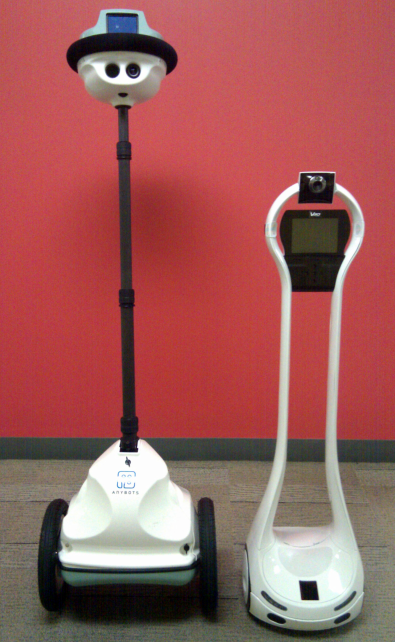
\includegraphics[scale=0.25]{Teleconference.png}
    \caption{Teleconference Robot}
    \label{Teleconference}
\end{figure}
    Figure.\ref{Teleconference} shows two telepresence robots capable of holding a teleconference, and they can be used widely in buildings, offices, conference rooms\cite{42}. Their big advantage is that they can make physical interaction or movement before or during the meeting, which makes the participates feel personally on the scene. The participates are able to express non-verbal behavior in addition to simply passing their audio and video data\cite{35}.
\par 
    Study has found that the level of a robot's presence affects the types of social interaction that people will engage with the robot\cite{43}. People feel more psychologically involved and more engaged in the interaction with their remote partners when they were embodied in a socially expressive way. When they're is using robot instead of computer or cell phone, they can achieve much higher levels of cooperation both on their own part and their partners as well as a higher score for enjoyment in the interaction. 
\par 
    Business and organizational meeting highly demands active participation from their members. Engagement in the interaction is important as well as cooperation. At meetings held by a teleconference robot, participants usually express more trust for the participates in the robot's screen and understand their words more clearly. In the case of cultural contact, evidence proves that a robot could improve the quality of connection\cite{44}. Participants will be more interested in meeting people from different cultures if the remote participant are introduced via a robot-based communication medium rather than with video conferencing technology. The participants seem to feel more positive, more familiar, and less inhibited interacting with the robot.
\par 
    The remote control system also makes users hold and attend meeting more safely and conveniently. In typical remote meeting, the discussion has to pause when the participates need to move or change the meeting place. However, telepresence robot make corridor a part of the meeting room. It doesn't require participates to be confined to a small, pre-determined area during meet. The robot's camera can use vision to extract the motion pattern of the human as well as the state of itself so that it can follow the movement of participates\cite{45}. In a business meeting where some products require demonstrations, the robot can provide a comprehensive viewing angle for the participates and deepen their understanding for the product. Since sometimes the robot is moving during a meeting, it supports dynamic volume control system. When in quiet room or noisy public area, the robot can adjust the volume according to its location.
\par 
    A study suggests that the robot do have a role to play in an office environment but perhaps not in the context of a formal meeting because formal meeting doesn't need much movement. It's believed that small and less formal meetings like stand up meetings seem to be the ideal scenario for teleconference robot. Experiment result shows that instead of using the robot in large formal meetings, it may have been more beneficial to assign a telepresence robot to the team in each hub to act as a portal.

\paragraph{Daily Application and Socialization}
    Robots have achieved satisfying performance in help people's daily routine and socialization, such as delivering food for them\cite{46}. After the outbreak of Covid-19, many infected patients were found in restaurants, hence they're mostly closed to prevent further infection. Under the circumstance, robots are used to deliver food. In some US states, AI's robot restaurant food delivery service has seen demand increase by four times since shut down\cite{47}.
\par 
    For people quarantined at home, the robot help them share time together and accompany each other remotely, which is very luxurious now. At present, some robots are being used to go shopping remotely\cite{48}. Consumers can view the products from the robot's camera, and pay money by showing QR code on the screen. During quarantine, the robot can either go to department store by itself as the substitute of consumer, or accompany friends to enhance socialization. In fact, robot shopping can be a new pattern for remote shopping. Compared to online shopping or remote shopping through a tablet, robot shopping gives the shopper a wider vision to view more goods at a time and gets more attention from the salesman\cite{49}. Experiment shows that the shopper tends to make different decisions when controlling a robot for remote shopping. 
\par 
    The embodiment of the telepresence robot creates a strong sense of presence of the controller, keeping people still be part of big moments in their lives during quarantine\cite{50}. It is reported that a father in quarantine control a telepresence robot to attend his daughter's wedding ceremony his daughter's wedding hundreds of kilometers away\cite{51}. He can see his daughter dancing from the robots screen. In some Asia schools, students are using telepresence robot to attend the graduate ceremony. Their faces were shown in the screen of the robot, and become part of their graduation photo together with diploma and trencher cap. 
\paragraph{Design Negligence}
    Like telepresence robot in hospitals and ICU, a robot's physical existence may also cause much inconvenience in the society. When they're moving freely, it may enter private space because of the controller's blind spot. In another occasion where the controller wanted to use the robot's arm to give audience a sign, it caused divergence and ambiguity in the understanding of the sign. Therefore, To design the robot properly, greater understanding about the real demands and situations of these application environments are required\cite{52}. The designer needs to consider not only the robot's appearance, but also finer interactions between a human and a robot. In addition, social interactions the impact of changes in physical presence should be investigated before choosing to replace a physical robot with a virtual or video-displayed agent. 
\paragraph{Requirement for Better Physical Contact}
    When it comes to business negotiation, many people believe that a negotiator who can not see their counterpart or make physical contact will be at a tactical disadvantage to their counterpart who can see them. In addition, physical contact is considered particularly important in interactions that demand mutual cooperation and trust\cite{53}. However, robots can't make physical contact as human. It need further improvement to make complex movements like human. For example, the shaking of hands was found to have a strong positive effect upon cooperation - as measured by mutually beneficial economic outcomes - when negotiators shook hands prior to commencing their negotiations. Up to now, only a few robots provide such physical contact, like stretch a hand with only one degree of freedom. In experiment, although most participants were able to overcome this awkwardness and grasp the hand fully, some chose instead to merely grasp the fingers of the hand instead. The result shows the feasibility for the physical contact provided by robots, but also reflects the fact that the robot still needs a lot of technological improvements to make the contact as natural as possible. 
\subsubsection{Educational Applications} 
    There are totally 7 articles focusing on Telepresence education robots, all being optimist about the future usage of the robot. All robots discussed in these articles were developed before the outbreak of Covid-19, aiming at providing students with remote access to school or lab. Figure.\ref{Education robot} shows three different Telepresence education robots, which have similar architecture and appearance to a normal telepresence robot. 
\begin{figure}[H]
    \centering
    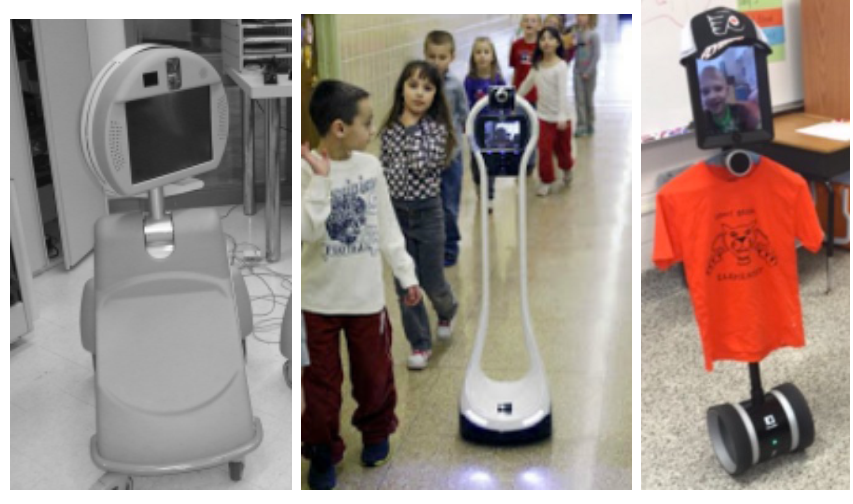
\includegraphics[scale=0.25]{Education.png}
    \caption{From left to right, PEBBLES, VGo, and Double
    Robots used in schools}
    \label{Education robot}
\end{figure}
    Telepresence education robots can be operated by both teachers or students in two scenarios. When the robot is controlled by a student, it will be put in the classroom. Student can control the robot through PC or tablet from home and watching the lecture. When the users are teachers, the robot will be set at student's home, controlled by teachers remotely. No matter who is the user, the video call and the mobile system supported by the robot enable teachers and students to communicate effectively in visual and audio.
\par 
    After the outbreak of Covid-19, many schools have started to provide online education. Student will stay home and attending class through online meeting software such as zoom through tablet or computer. Telepresence education robots is another option for student to attend to school during quarantine. Compared to normal online meeting software, Telepresence education robots have more features and functions. Studies also show that these robots can improve the quality of online education.
\paragraph{Education Quality Improvement}
    A Telepresence education robot called Engkey can track the head and facial features of people, then it can imitate these features\cite{54}. In classroom, Engkey can arouse students' interest and attention in learning and interacting with the teacher because they can understand each other's emotion and feedback better. In addition, socialization with others is an important learning experience of being at school, and it is part of the education\cite{55}. Telepresence education robot can provide students physical and social contact with each other by moving around or raising an arm. Interaction through robots help students overcome isolation at home to meet their social emotional needs\cite{56}.
\paragraph{Remote Lab}
    For senior students or researchers, research at lab is necessary, and sometimes it can't be interrupt by external factors. A system consisted of telepresence robot and smart lab were developed help these people do research remotely\cite{57}. It is shown that users succeed in making simple experiments and picking up equipments by operating the system remotely.
\begin{figure}[H]
    \centering
    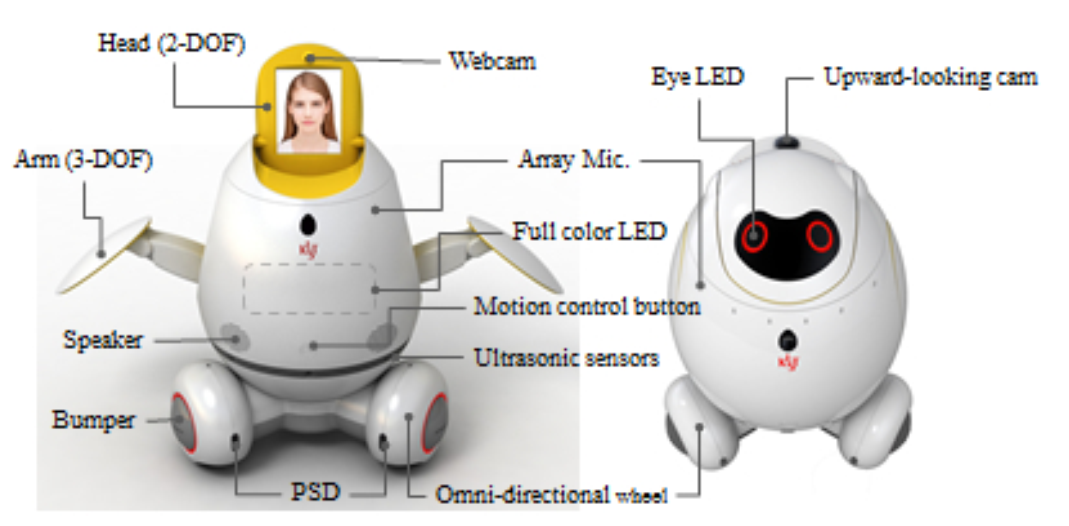
\includegraphics[scale=0.25]{Engkey.png}
    \caption{System overview of Engkey}
    \label{Engkey}
\end{figure}
    According to interview with teachers, students, and their families, telepresence education robot can provide better experience than video call in remote education. The robot's control and navigation system is smooth enough for user to move the robot and interact with external environment. The cost of these robots and prototypes is reasonable, ranging from 400\$ to 6000\$, which is cheaper than inviting a private teacher to home. When the pandemic is over, these Telepresence education robot can still be used by disabled students. It's also a good option for researchers who need to work under a dangerous environment.
    
\paragraph{Difficult User Interface}
    Telepresence education robot shares similar drawbacks from normal telepresence robot, but it need more improvements from education purpose. The narrow view and camera with low resolution is often complained by many users\cite{58}. Sometimes they can't check obstacles at near position due to the limitation of camera and the low resolution may reduce eye contact between teacher and students, which is an important factor for education.\cite{59}.  It is also reported that teachers are worried to interrupt or affect the class because touch the wrong button on the robot. They are also afraid of being responsible for damaging the robots unexpectedly while parents are worried that home privacy will be exposed when the robot are being remotely controlled. Besides, some students feel pain in fingers after using the robot for a long time\cite{60}. To make full use of the Telepresence education robot, developers need to improve the mechanic structure and user interface from the view of teachers and students.  The robot's user interface must be user friendly as much as possible to ensure the high education quality. For example, the developers should add another screen on the robot so that the users can see the other's face and the textbook at the same time.
\paragraph{Lack of Standard}  
    On the other hand, like robots used in hospitals, telepresence education robots also require clear criteria, especially when the user is children. To alleviate concerns, the criteria should include user manual, accident management, safety standard, and etc. Users will only acquire fully control of the robot after completing the whole tutoring and training class.
\paragraph{More Functions}
    Some articles mention that more functions can greatly improve the practicability of Telepresence education robots. According to teachers' feedback, if the robot can have or be connected to another camera which can cover the entire view of the class, they give a better lecture. On the other hand, some controllers consider autonomous moving function very helpful because they feel trouble to keep controlling the movement of robot and avoiding collision. This function frees them from driving the robot and allows them to focus on the content in the screen and interacting with the teacher and classmates.
\paragraph{One-to-N Control}
    All robots discussed in the articles adopt one-to-one control system, which means one user can only control one robot at a time. However, it is possible that a robot is controlled by more people collaboratively and one controller is operating multiple robots. On this occasion, teachers can teach a lesson to many students at the same time by synchronously control many robots through one control system. Compared to teach students one on one, synchronously control system can greatly reduce teacher's burden. For student controllers, if they're going to control a robot with peers together, they can learn more experience about team work and socialization.
\subsubsection{Industrial Applications}
    There are 3 news reports specially focusing on the robot's role in industry. These robots work in the factory or other areas to improve the production of medical resources. 
\paragraph{Intelligent Automation} 
    Industrial robots apply artificial intelligence and cloud technology to work collaboratively and automatically. In China, where the disease was first detected, medicine and food delivery robots have done a great job in transporting essential supplies between healthy facilities. In airport industry, AI-enabled bot automatically extracts ticket information from customer data on file, opens an airline's booking and refund applications, and issues an e-voucher for future travel. By applying machine learning and natural language processing, most refund requests are being handled in roughly three minutes, down from about 20 minutes by agents. In recycling industry, MP Robotics in Colorado had a big increase in orders for its robots using artificial intelligence to examine recycled material, removing garbage\cite{61}. 
\par 
    These advanced industrial robots don't need human's regulation but can work at a higher efficiency. They represent the future of industrial automation system, which is unmanned and more flexible. Under pandemic, they help maintain social distancing between workers to reducing the chances for spreading disease. 
\paragraph{Quick reaction} 
    More importantly, when there is a emergency demand hike for certain products like protection suits or masks, these industrial robots can be easily mobilized to manufacture them and reduce manufacturers' pressure. Warehouse robot can pack and transport materials in warehouses, factories and distribution centers\cite{62}. They can reduce time and cost for transportation of essential materials. Cobot, a robot developed to co-work with people together, can help manufacture medical ventilators\cite{63}. Cobot can decrease man-hours required to produce each ventilator by automating nearly half of the processes required for ventilator assembly. It is also reported that Fetch Robotics', a robot company, has received 63\% more inquiries for industrial robots from different manufacturers' since the outbreak of Covid-19. 
\paragraph{Obstacles to Popularization}
    Unlike other robots, the primarily users and developers of these advanced industrial robots are big business companies and manufacturers like Amazon. To defend its market share, the company may be unwilling to share the technology at a low price because such technology may help their competitors and improve their productivity. The competition between companies may prevent the advanced industrial robots from being used at large scale. 
\par 
    On the other hand, it requires technical talents to operate and maintain these precise robots, which is very difficult for manufacturers in developing area. Since Covid-19 is a global pandemic, there are many people and companies from poor areas suffering greatly from the disease, but lack of money and technology make it impossible for these companies to take advantage of these robots because. 
\par 
    To popularize advanced industrial robots, the government need to facilitate the construction of infrastructures, like 5G station. On the manufacturer side, they can try to develop a simplified and modified version of industrial robot with lower cost. Even for a robot with a few functions, such as transportation, has already been proved very practical and can still offer great help in improving productivity.
\section{Conclusion}
    This systematic review has collected information about robots developed before and after the outbreak of Covid-19 and classify them into four categories according to their feasible applications. The review highlights the robots' performance and potential during pandemic and points out their short shortcomings. Among all these robots, telepresence robot is playing an outstanding role in helping fighting against Covid-19, thanks to its immune to the virus as well as real-time remote control system. With more and more robots being developed and applied during pandemic, Covid-19 brings a opportunity for hospitals, companies and schools to have a trial on large scale us of robots. It may stimulate the revolution and development of robots' modern application. 
    \par The review enable possible users to generate a deep understanding of robots for Covid-19 management, and help them to select the best robot according to their requirements. For developers, the systematic review provides valuable feedback and analysis about the drawbacks of robots. The feedback and analysis are from different perspectives, ranging from user experience, social acceptance, design issues, and etc. Then, the suggestions given by the review can offer help for further improvement.
\section{Study Limitations}
The content of this systematic review is highly limited to the keywords for search. Therefore, there are other areas where the robot can come into play but are not covered by the review. In terms of publish time, all the studies and articles covered by the review are published from 2010 to 2020, so it may omit some valuable information contained in articles published earlier. Since the outbreak of Covid-19 is not long ago, some related studies and reports have not been published, and they're also not covered by this review. 
\par Futhermore, among all articles covered, there are only a few providing a comprehensive introduction and analysis on a specific robot which is already put into use. As a result, the review can only propose universal ideas about robots, which are based on fragmented information from many articles.
\begin{thebibliography}{99} 
    \bibitem{1}https://covid19.who.int/ 2020/6/2, 10:06am CEST
    \bibitem{2}World Economic Outlook, April 2020: The Great Lockdown https://www.imf.org/en/Publications/WEO/Issues/2020/04/14/weo-april-2020
    \bibitem{99}D. Moher, A. Liberati, J. Tetzlaff, and D.G. Altman,Preferred reporting items for systematic reviews and meta-analyses: the PRISMA statement, Annals of Internal Medicine, vol. 151, no. 4, 2009, pp. 264–269
    \bibitem{3}Aggarwal, S., et al. (2019). A Literature Survey on Robotics in healthcare. 2019 4th International Conference on Information Systems and Computer Networks (ISCON).
    \bibitem{4}Carranza, K. A. R., et al. (2018). Akibot: A Telepresence Robot for Medical Teleconsultation. 2018 IEEE 10th International Conference on Humanoid, Nanotechnology, Information Technology,Communication and Control, Environment and Management (HNICEM).
    \bibitem{5}Burke, R. V., et al. (2012). "Using robotic telecommunications to triage pediatric disaster victims." Journal of Pediatric Surgery 47(1): 221-224.
    \bibitem{6}Lepage, P., et al. (2016). Telehomecare telecommunication framework — From remote patient monitoring to video visits and robot telepresence. 2016 38th Annual International Conference of the IEEE Engineering in Medicine and Biology Society (EMBC).
    \bibitem{7}J, P., et al. (2016). Telepresence Robot Doctor. 2016 Online International Conference on Green Engineering and Technologies (IC-GET).
    \bibitem{8}Translated by ContentEngine, L. L. C. (2020). Robot consultation with Covid-19 patients. CE Noticias Financieras. Miami.
    \bibitem{9}Loten, A. (2020). Calling All Robots: Businesses Automate the Battle Against Coronavirus; Hospital workers are using software robots to track Covid-19 tests. Wall Street Journal (Online). New York, N.Y.
    \bibitem{10}Vespa, P. (2005). "Robotic telepresence in the intensive care unit." Critical Care 9(4): 319-320.
    \bibitem{11}Becevic, M., et al. (2015). "Robotic Telepresence in a Medical Intensive Care Unit--Clinicians' Perceptions." Perspectives in health information management 12: 1c.
    \bibitem{12}Sucher, J. F., et al. (2011). "Robotic telepresence: a helpful adjunct that is viewed favorably by critically ill surgical patients." American Journal of Surgery 202(6): 0-847.
    \bibitem{13}Reynolds, E. M., et al. (2012). "Utilization of robotic "remote presence" technology within North American intensive care units." Telemedicine journal and e-health : the official journal of the American Telemedicine Association 18(7): 507-515.
    \bibitem{14}Falleni, S., et al. (2017). Teleoperated multimodal robotic interface for telemedicine: A case study on remote auscultation. 2017 26th IEEE International Symposium on Robot and Human Interactive Communication (RO-MAN).
    \bibitem{15}Hai, N. D. X., et al. (2019). Remote healthcare for the Elderly, Patients by Tele-Presence Robot. 2019 International Conference on System Science and Engineering (ICSSE).
    \bibitem{16}Briere, S., et al. (2009). In-home telehealth clinical interaction using a robot.
    \bibitem{17}Zhou, B., et al. (2018). "A New Remote Health-Care System Based on Moving Robot Intended for the Elderly at Home." Journal of healthcare Engineering.
    \bibitem{18}Su, C., et al. (2018). Doctor Robot with Physical Examination for Skin Disease Diagnosis and Telemedicine Application. 2018 International Conference on System Science and Engineering (ICSSE).
    \bibitem{19}Hedge, Z. (2020). "Phil's Stock World: “Meet The Global Robot Army That’s Been Deployed To Fight COVID-19."  
    \bibitem{20}Loten, A. (2020). Travel Industry Automates Pandemic Response With New Digital Tools; A fever-detecting camera that screens travelers and a hotel-room cleaning robot join the industry's front-line workers. Wall Street Journal (Online). New York, N.Y.
	\bibitem{21}Shaaban, A. (2020). This robot can remotely detect Covid-19 patients. TCA Regional News. Chicago.
	\bibitem{22}Translated by ContentEngine, L. L. C. (2020). Ready first Mexican robot 'nurse' against Covid-19. CE Noticias Financieras. Miami.
    \bibitem{23}Translated by ContentEngine, L. L. C. (2020). "RoomieBot": First Mexican healthcare robot ready to identify suspected Covid-19 cases in hospitals. CE Noticias Financieras. Miami.
    \bibitem{24}Gonzalez-Jimenez, J., et al. (2013). Evaluation of a Telepresence Robot for the Elderly: A Spanish Experience.
    \bibitem{25}Cesta, A., et al. (2012). ADDRESSING THE LONG-TERM EVALUATION OF A TELEPRESENCE ROBOT FOR THE ELDERLY.
    \bibitem{26}Bugtai, N. T., et al. (2017). Development of a Telepresence Robot for Medical Consultation. Biomedical Engineering's
    \bibitem{33}Laniel, S., et al. (2017). Adding navigation, artificial audition and vital sign monitoring capabilities to a telepresence mobile robot for remote home care applications. 2017 International Conference on Rehabilitation Robotics (ICORR).
    \bibitem{27}Lee, H., et al. (2017). Assessment of user needs for the teleconsultation robot and the bedside robot using simulation. 2017 International Conference on Intelligent Informatics and Biomedical Sciences (ICIIBMS).
	\bibitem{28}Bettinelli, M., et al. (2015). "Does Robotic Telerounding Enhance Nurse-Physician Collaboration Satisfaction About Care Decisions?" Telemedicine journal and e-health : the official journal of the American Telemedicine Association 21(8): 637-643.
    \bibitem{31}Sinharay, A., et al. (2016). A Novel Approach to Unify Robotics, Sensors, and Cloud Computing Through IoT for a Smarter healthcare Solution for Routine Checks and Fighting Epidemics. Internet of Things: Iot Infrastructures, Pt I. B. Mandler, J. MarquezBarja, M. E. M. Campista et al. 169: 536-542.
    \bibitem{32}Laniel, S., et al. (2017). Adding navigation, artificial audition and vital sign monitoring capabilities to a telepresence mobile robot for remote home care applications. 2017 International Conference on Rehabilitation Robotics (ICORR).
    \bibitem{34}Express, C. (2020). "How robots can help combat the coronavirus pandemic." Express Computer.
    \bibitem{29}Kraft, K. and W. D. Smart (2016). Seeing is comforting: Effects of teleoperator visibility in robot-mediated healthcare. 2016 11th ACM/IEEE International Conference on Human-Robot Interaction (HRI).
    \bibitem{30}Frennert, S. A., et al. (2013). "Elderly People's Perceptions of a Telehealthcare System: Relative Advantage, Compatibility, Complexity and Observability."  31(3): 218-237.
    
    \bibitem{36}Siddiqui, H. (2020). Coronavirus: Use of autonomous robot for law enforcement during COVID-19 lockdown. Financial Express. New Delhi.
    \bibitem{37}Translated by ContentEngine, L. L. C. (2020). Boston Dynamics uses its robots in a hospital to protect health workers from Covid-19. CE Noticias Financieras. Miami.
    \bibitem{38}Translated by ContentEngine, L. L. C. (2020). Robot dog looking to prevent the spread of Covid-19 in Singapore. CE Noticias Financieras. Miami.
    \bibitem{39}Minj, V. (2020). Robots At Duty To Prevent Spread of COVID-19 Infection. Electronics for You. New Delhi, Athena Information Solutions Pvt. Ltd.
    \bibitem{40}Karnad, N. and V. Isler (2010). A multi-robot system for unconfined video-conferencing. 2010 IEEE International Conference on Robotics and Automation.
    \bibitem{41}Tsui, K. M., et al. (2011). Exploring use cases for telepresence robots. 2011 6th ACM/IEEE International Conference on Human-Robot Interaction (HRI).
    \bibitem{42}Choi, D.-W., et al. (2011). Design the Video Conferencing Robot for One-to-Many Communication using Smartphone.
    \bibitem{35}Adalgeirsson, S. O. and C. Breazeal (2010). MeBot: A robotic platform for socially embodied telepresence. 2010 5th ACM/IEEE International Conference on Human-Robot Interaction (HRI).
    \bibitem{43}Bainbridge, W. A., et al. (2011). "The Benefits of Interactions with Physically Present Robots over Video-Displayed Agents." International Journal of Social Robotics 3(1): 41-52.
    \bibitem{44}Kim, N., et al. (2014). Is a Robot Better than Video for Initiating Remote Social Connections Among Children? Hri'14: Proceedings of the 2014 Acm/Ieee International Conference on Human-Robot Interaction: 208-209.
    \bibitem{45}Kanigoro, B., et al. (2014). "Web based conference system for intelligence telepresence robot: a framework." Journal of Computer Science 10(1): 10-14.
    \bibitem{46}Buzalka, M. (2020). "5 coronavirus things: Meal delivery robots help minimize COVID spread at University of Wisconsin." Food Management.
    \bibitem{47}Payne, H. (2020). Robots on the rise in the COVID-19 economy. TCA Regional News. Chicago.
	\bibitem{48}Translated by ContentEngine, L. L. C. (2020). Student creates robot to take to the streets and make purchases during pandemic. CE Noticias Financieras. Miami.
    \bibitem{49}Yang, L., et al. (2018). "Shopping Over Distance through a Telepresence Robot." Proceedings of the ACM on Human-Computer Interaction 2(CSCW): 191 (118 pp.)-191 (118 pp.).
    \bibitem{50}Lillian, Y. and C. Neustaedter (2018). "Our House: Living Long Distance with a Telepresence Robot." Proceedings of the ACM on Human-Computer Interaction 2(CSCW): 190 (118 pp.)-190 (118 pp.).
    \bibitem{51}Quinn, M. (2020). A Father in Quarantine, a Wedding and a Robot. Washington, Federal Information \& News Dispatch, LLC.
    \bibitem{52}Lee, H., et al. (2016). Designing the Appearance of a Telepresence Robot, M4K: A Case Study. Cultural Robotics, Cr 2015. J. Koh, B. J. Dunstan, D. SilveraTawil and M. Velonaki. 9549: 33-43.
    \bibitem{53}Bevan, C. and D. S. Fraser (2015). Shaking Hands and Cooperation in Tele-present Human-Robot Negotiation. 2015 10th ACM/IEEE International Conference on Human-Robot Interaction (HRI)
    \bibitem{54}Yun, S., et al. (2011). "Engkey: Tele-education Robot."
    \bibitem{55}Bloss, R. (2011). "High school student goes to class robotically." The Industrial Robot 38(5): 465-468.
    \bibitem{56}Newhart, V. A., et al. (2016). "Virtual Inclusion via Telepresence Robots in the Classroom: An Exploratory Case Study." International Journal of Technologies in Learning 23(4): 9-25.
    \bibitem{57}Qing, T., et al. (2019). "Toward a telepresence robot empowered smart lab." Smart Learning Environments 6(1): 5 (19 pp.)-15 (19 pp.).
    \bibitem{58}Lim, M. and H. Jeong-Hye (2019). "Convergence Technologies by a Long-term Case Study on Telepresence Robot-assisted Learning." Journal of Convergence for Information Technology 9(7): 106-113.
    \bibitem{59}Oh-Hun, K., et al. (2010). Telepresence robot system for English tutoring. 2010 IEEE Workshop on Advanced Robotics and its Social Impacts.
    \bibitem{60}Newhart, V. A., et al. (2017). My Student is a Robot: How Schools Manage Telepresence Experiences for Students.
    \bibitem{61}Translated by ContentEngine, L. L. C. (2020). Coronavirus: pandemic accelerates automatism and robot requests soar. CE Noticias Financieras. Miami.
    \bibitem{62}Seitz, P. (2020). Covid-19 Crisis Could Be Time For Warehouse Robots To Shine. Investor's Business Daily. Los Angeles.
    \bibitem{63}Ali Ahmad, M., et al. (2020). Reconfiguring and ramping-up ventilator production in the face of COVID-19: Can robots help? Ithaca, Cornell University Library, arXiv.org.
\end{thebibliography}
\end{document}